% !TEX root = ../report.tex

\chapter{Конструкторская часть}

В данном разделе производится формализация сущностей базы данных, описываются столбцы таблиц и ограничения целостности. Устанавливается ролевая модель доступа на уровне СУБД, проектируются триггеры и хранимая функция. Проводится проверка соответствия спроектированной базы данных третьей нормальной форме.

% !TEX root = ../../report.tex

\section{Описание сущностей базы данных}

В соответствии с таблицей~\ref{tbl:entities}, описывающей сущности предметной области, выделяются следующие таблицы:

\begin{itemize}
    \item users --- таблица пользователей;
    \item sellers --- таблица продавцов;
    \item products --- таблица товаров;
    \item categories --- таблица категорий;
    \item product\_categories --- таблица связей товаров и категорий;
    \item addresses --- таблица адресов доставки;
    \item orders --- таблица заказов;
    \item order\_items --- таблица позиций заказов;
    \item reviews --- таблица отзывов;
    \item product\_price\_history --- таблица истории изменения цен.
\end{itemize}

В таблицах~\ref{tbl:t_users}--\ref{tbl:t_price_history} приведены столбцы и их ограничения для каждой из перечисленных таблиц.

\begin{table}[H]
    \caption{Описание столбцов таблицы users}
    \label{tbl:t_users}
    \begin{tabular}[]{|c|c|c|c|}
        \hline
        \textbf{Столбец} & \textbf{Тип данных} & \textbf{Ограничения} & \textbf{Описание} \\ \hline
        id & BIGSERIAL & \makecell{NOT NULL \\ PRIMARY KEY} & идентификатор \\ \hline
        email & VARCHAR(255) & \makecell{NOT NULL \\ UNIQUE} & электронная почта \\ \hline
        password\_hash & VARCHAR(255) & NOT NULL & хеш пароля \\ \hline
        full\_name & VARCHAR(255) & NOT NULL & полное имя \\ \hline
        phone & VARCHAR(20) & --- & номер телефона \\ \hline
        role & VARCHAR(20) & \makecell{NOT NULL \\ CHECK} & \makecell{роль: buyer, seller,\\admin, analyst} \\ \hline
        created\_at & TIMESTAMPTZ & \makecell{NOT NULL \\ DEFAULT now()} & дата создания \\ \hline
        deleted\_at & TIMESTAMPTZ & --- & \makecell{дата мягкого\\удаления} \\ \hline
    \end{tabular}
\end{table}

\begin{table}[H]
    \caption{Описание столбцов таблицы sellers}
    \label{tbl:t_sellers}
    \begin{tabular}[]{|c|c|c|c|}
        \hline
        \textbf{Столбец} & \textbf{Тип данных} & \textbf{Ограничения} & \textbf{Описание} \\ \hline
        id & BIGSERIAL & \makecell{NOT NULL \\ PRIMARY KEY} & идентификатор \\ \hline
        user\_id & BIGINT & \makecell{NOT NULL \\ UNIQUE \\ FOREIGN KEY} & \makecell{ссылка на\\пользователя} \\ \hline
        company\_name & VARCHAR(255) & NOT NULL & название компании \\ \hline
        description & TEXT & --- & описание \\ \hline
        rating & NUMERIC(3,2) & --- & \makecell{рейтинг\\(пересчитывается\\триггером)} \\ \hline
        created\_at & TIMESTAMPTZ & \makecell{NOT NULL \\ DEFAULT now()} & дата создания \\ \hline
    \end{tabular}
\end{table}

\begin{table}[H]
    \caption{Описание столбцов таблицы products}
    \label{tbl:t_products}
    \begin{tabular}[]{|c|c|c|c|}
        \hline
        \textbf{Столбец} & \textbf{Тип данных} & \textbf{Ограничения} & \textbf{Описание} \\ \hline
        id & BIGSERIAL & \makecell{NOT NULL \\ PRIMARY KEY} & идентификатор \\ \hline
        seller\_id & BIGINT & \makecell{NOT NULL \\ FOREIGN KEY} & \makecell{ссылка на\\продавца} \\ \hline
        name & VARCHAR(255) & NOT NULL & название товара \\ \hline
        description & TEXT & --- & описание \\ \hline
        price & NUMERIC(12,2) & \makecell{NOT NULL \\ CHECK $> 0$} & цена \\ \hline
        stock\_quantity & INTEGER & \makecell{NOT NULL \\ CHECK $\geq 0$ \\ DEFAULT 0} & \makecell{количество\\на складе} \\ \hline
        reserved\_quantity & INTEGER & \makecell{NOT NULL \\ CHECK $\geq 0$ \\ DEFAULT 0 \\ CHECK $\leq$\\stock\_quantity} & \makecell{количество\\в резерве} \\ \hline
        rating & NUMERIC(3,2) & --- & \makecell{рейтинг\\(пересчитывается\\триггером)} \\ \hline
        created\_at & TIMESTAMPTZ & \makecell{NOT NULL \\ DEFAULT now()} & дата создания \\ \hline
        deleted\_at & TIMESTAMPTZ & --- & \makecell{дата мягкого\\удаления} \\ \hline
    \end{tabular}
\end{table}

\begin{table}[H]
    \caption{Описание столбцов таблицы categories}
    \label{tbl:t_categories}
    \begin{tabular}[]{|c|c|c|c|}
        \hline
        \textbf{Столбец} & \textbf{Тип данных} & \textbf{Ограничения} & \textbf{Описание} \\ \hline
        id & BIGSERIAL & \makecell{NOT NULL \\ PRIMARY KEY} & идентификатор \\ \hline
        parent\_id & BIGINT & FOREIGN KEY & \makecell{ссылка на\\родительскую\\категорию} \\ \hline
        name & VARCHAR(255) & \makecell{NOT NULL \\ UNIQUE} & название категории \\ \hline
        description & TEXT & --- & описание \\ \hline
    \end{tabular}
\end{table}

\begin{table}[H]
    \caption{Описание столбцов таблицы product\_categories}
    \label{tbl:t_product_categories}
    \begin{tabular}[]{|c|c|c|c|}
        \hline
        \textbf{Столбец} & \textbf{Тип данных} & \textbf{Ограничения} & \textbf{Описание} \\ \hline
        product\_id & BIGINT & \makecell{NOT NULL \\ FOREIGN KEY} & \makecell{ссылка на\\товар} \\ \hline
        category\_id & BIGINT & \makecell{NOT NULL \\ FOREIGN KEY} & \makecell{ссылка на\\категорию} \\ \hline
        \multicolumn{4}{|c|}{PRIMARY KEY (product\_id, category\_id)} \\ \hline
    \end{tabular}
\end{table}

\begin{table}[H]
    \caption{Описание столбцов таблицы addresses}
    \label{tbl:t_addresses}
    \begin{tabular}[]{|c|c|c|c|}
        \hline
        \textbf{Столбец} & \textbf{Тип данных} & \textbf{Ограничения} & \textbf{Описание} \\ \hline
        id & BIGSERIAL & \makecell{NOT NULL \\ PRIMARY KEY} & идентификатор \\ \hline
        user\_id & BIGINT & \makecell{NOT NULL \\ FOREIGN KEY} & \makecell{ссылка на\\пользователя} \\ \hline
        city & VARCHAR(100) & NOT NULL & город \\ \hline
        street & VARCHAR(255) & NOT NULL & улица \\ \hline
        house & VARCHAR(20) & NOT NULL & дом \\ \hline
        apartment & VARCHAR(20) & --- & квартира \\ \hline
        zip\_code & VARCHAR(20) & NOT NULL & почтовый индекс \\ \hline
        is\_default & BOOLEAN & \makecell{NOT NULL \\ DEFAULT false} & \makecell{признак основного\\адреса} \\ \hline
        created\_at & TIMESTAMPTZ & \makecell{NOT NULL \\ DEFAULT now()} & дата создания \\ \hline
    \end{tabular}
\end{table}

\begin{table}[H]
    \caption{Описание столбцов таблицы orders}
    \label{tbl:t_orders}
    \begin{tabular}[]{|c|c|c|c|}
        \hline
        \textbf{Столбец} & \textbf{Тип данных} & \textbf{Ограничения} & \textbf{Описание} \\ \hline
        id & BIGSERIAL & \makecell{NOT NULL \\ PRIMARY KEY} & идентификатор \\ \hline
        user\_id & BIGINT & \makecell{NOT NULL \\ FOREIGN KEY} & \makecell{ссылка на\\покупателя} \\ \hline
        seller\_id & BIGINT & \makecell{FOREIGN KEY \\ (nullable)} & \makecell{ссылка на продавца\\(заполняется при\\оформлении)} \\ \hline
        address\_id & BIGINT & \makecell{FOREIGN KEY \\ (nullable)} & \makecell{ссылка на адрес\\(null для\\корзины-черновика)} \\ \hline
        status & VARCHAR(30) & \makecell{NOT NULL \\ CHECK} & \makecell{статус: draft,\\pending, paid,\\shipped, delivered,\\cancelled} \\ \hline
        total\_amount & NUMERIC(12,2) & \makecell{NOT NULL \\ CHECK $\geq 0$} & итоговая сумма \\ \hline
        created\_at & TIMESTAMPTZ & \makecell{NOT NULL \\ DEFAULT now()} & дата создания \\ \hline
        updated\_at & TIMESTAMPTZ & \makecell{NOT NULL \\ DEFAULT now()} & дата обновления \\ \hline
    \end{tabular}
\end{table}

\begin{table}[H]
    \caption{Описание столбцов таблицы order\_items}
    \label{tbl:t_order_items}
    \begin{tabular}[]{|c|c|c|c|}
        \hline
        \textbf{Столбец} & \textbf{Тип данных} & \textbf{Ограничения} & \textbf{Описание} \\ \hline
        id & BIGSERIAL & \makecell{NOT NULL \\ PRIMARY KEY} & идентификатор \\ \hline
        order\_id & BIGINT & \makecell{NOT NULL \\ FOREIGN KEY} & ссылка на заказ \\ \hline
        product\_id & BIGINT & \makecell{NOT NULL \\ FOREIGN KEY} & ссылка на товар \\ \hline
        quantity & INTEGER & \makecell{NOT NULL \\ CHECK $> 0$} & количество \\ \hline
        price\_at\_purchase & NUMERIC(12,2) & \makecell{NOT NULL \\ CHECK $> 0$} & \makecell{цена на момент\\покупки} \\ \hline
        \multicolumn{4}{|c|}{UNIQUE (order\_id, product\_id)} \\ \hline
    \end{tabular}
\end{table}

\begin{table}[H]
    \caption{Описание столбцов таблицы reviews}
    \label{tbl:t_reviews}
    \begin{tabular}[]{|c|c|c|c|}
        \hline
        \textbf{Столбец} & \textbf{Тип данных} & \textbf{Ограничения} & \textbf{Описание} \\ \hline
        id & BIGSERIAL & \makecell{NOT NULL \\ PRIMARY KEY} & идентификатор \\ \hline
        user\_id & BIGINT & \makecell{NOT NULL \\ FOREIGN KEY} & \makecell{ссылка на\\пользователя} \\ \hline
        product\_id & BIGINT & \makecell{NOT NULL \\ FOREIGN KEY} & ссылка на товар \\ \hline
        rating & SMALLINT & \makecell{NOT NULL \\ CHECK 1..5} & оценка от 1 до 5 \\ \hline
        comment & TEXT & --- & текст отзыва \\ \hline
        created\_at & TIMESTAMPTZ & \makecell{NOT NULL \\ DEFAULT now()} & дата создания \\ \hline
        \multicolumn{4}{|c|}{UNIQUE (user\_id, product\_id)} \\ \hline
    \end{tabular}
\end{table}

\begin{table}[H]
    \caption{Описание столбцов таблицы product\_price\_history}
    \label{tbl:t_price_history}
    \begin{tabular}[]{|c|c|c|c|}
        \hline
        \textbf{Столбец} & \textbf{Тип данных} & \textbf{Ограничения} & \textbf{Описание} \\ \hline
        id & BIGSERIAL & \makecell{NOT NULL \\ PRIMARY KEY} & идентификатор \\ \hline
        product\_id & BIGINT & \makecell{NOT NULL \\ FOREIGN KEY} & ссылка на товар \\ \hline
        old\_price & NUMERIC(12,2) & NOT NULL & старая цена \\ \hline
        new\_price & NUMERIC(12,2) & NOT NULL & новая цена \\ \hline
        changed\_at & TIMESTAMPTZ & \makecell{NOT NULL \\ DEFAULT now()} & дата изменения \\ \hline
        changed\_by & TEXT & \makecell{NOT NULL \\ DEFAULT\\current\_user} & \makecell{инициатор\\изменения} \\ \hline
    \end{tabular}
\end{table}

Помимо первичных ключей и ограничений уникальности, для оптимизации запросов создаются дополнительные индексы. Перечень индексов приведён в таблице~\ref{tbl:indexes}.

\begin{table}[H]
    \caption{Индексы базы данных}
    \label{tbl:indexes}
    \begin{tabular}{|l|l|l|}
        \hline
        \textbf{Индекс} & \textbf{Столбцы} & \textbf{Назначение} \\ \hline
        \makecell[l]{idx\_products\_\\seller\_id} & \makecell[l]{products\\(seller\_id)} & \makecell[l]{выборка товаров\\продавца} \\ \hline
        \makecell[l]{idx\_orders\_\\user\_id} & \makecell[l]{orders\\(user\_id)} & \makecell[l]{выборка заказов\\покупателя} \\ \hline
        \makecell[l]{ux\_orders\_one\_\\draft\_per\_user} & \makecell[l]{orders\\(user\_id)\\WHERE status = 'draft'} & \makecell[l]{единственная\\корзина покупателя} \\ \hline
        \makecell[l]{idx\_orders\_\\status\_created\_at} & \makecell[l]{orders\\(status, created\_at)} & \makecell[l]{фильтрация заказов\\по статусу и дате} \\ \hline
        \makecell[l]{idx\_product\_\\categories\_\\category\_id} & \makecell[l]{product\_categories\\(category\_id)} & \makecell[l]{выборка товаров\\по категории} \\ \hline
        \makecell[l]{idx\_reviews\_\\product\_id} & \makecell[l]{reviews\\(product\_id)} & \makecell[l]{выборка отзывов\\на товар} \\ \hline
        \makecell[l]{idx\_products\_\\id\_not\_deleted} & \makecell[l]{products (id)\\WHERE deleted\_at\\IS NULL} & \makecell[l]{частичный индекс:\\только активные\\товары} \\ \hline
        \makecell[l]{idx\_users\_\\id\_not\_deleted} & \makecell[l]{users (id)\\WHERE deleted\_at\\IS NULL} & \makecell[l]{частичный индекс:\\только активные\\пользователи} \\ \hline
        \makecell[l]{idx\_products\_\\price} & \makecell[l]{products\\(price)} & \makecell[l]{сортировка и\\фильтрация по цене} \\ \hline
    \end{tabular}
\end{table}

Частичные индексы (\texttt{WHERE deleted\_at IS NULL}) обеспечивают эффективный поиск только среди активных записей, исключая мягко удалённые строки из индексного дерева.

\clearpage


% !TEX root = ../../report.tex

\section{Ролевая модель}

Ролевая модель используется для разграничения доступа к таблицам базы данных на уровне СУБД. Каждой роли назначается набор привилегий, определяющий допустимые операции.

В аналитической части были определены пять ролей пользователей системы. На уровне СУБД проектируются четыре роли, соответствующие авторизованным пользователям. Роль гостя не выделяется как отдельная роль СУБД, поскольку действия гостя ограничиваются просмотром общедоступных данных и авторизацией. Просмотр гостем общедоступных данных соответствует чтению каталога, карточек продавцов, отзывов и истории цен.

Описание привилегий каждой роли приведено ниже.

\textbf{marketplace\_buyer} --- роль покупателя:
\begin{itemize}
    \item чтение таблиц products, sellers, categories, product\_categories, reviews, product\_price\_history --- просмотр каталога, карточек товаров, продавцов, отзывов и истории цен;
    \item управление таблицами addresses, reviews, orders, order\_items --- работа с адресами, отзывами, заказами и позициями заказа.
\end{itemize}

\textbf{marketplace\_seller} --- роль продавца:
\begin{itemize}
    \item управление таблицами sellers, products, product\_categories --- работа с профилем продавца, товарами и их категориями;
    \item чтение таблиц categories, reviews, product\_price\_history --- просмотр категорий, отзывов и истории цен;
    \item чтение таблиц orders и order\_items, обновление таблицы orders --- просмотр заказов продавца и фиксация статусов отгрузки и доставки.
\end{itemize}

\textbf{marketplace\_admin} --- роль администратора:
\begin{itemize}
    \item управление всеми таблицами --- полный доступ к данным.
\end{itemize}

\textbf{marketplace\_analyst} --- роль аналитика:
\begin{itemize}
    \item чтение всех таблиц --- доступ к данным без возможности модификации.
\end{itemize}

Сводная таблица привилегий ролей приведена в таблице~\ref{tbl:role_matrix}.

\begin{table}[H]
    \caption{Матрица привилегий ролей}
    \label{tbl:role_matrix}
    \begin{tabular}{|l|c|c|c|c|}
        \hline
        \textbf{Таблица} & \textbf{buyer} & \textbf{seller} & \textbf{admin} & \textbf{analyst} \\ \hline
        users & --- & --- & CRUD & R \\ \hline
        sellers & R & CRUD & CRUD & R \\ \hline
        products & R & CRUD & CRUD & R \\ \hline
        categories & R & R & CRUD & R \\ \hline
        product\_categories & R & CRUD & CRUD & R \\ \hline
        addresses & CRUD & --- & CRUD & R \\ \hline
        orders & CRUD & RU & CRUD & R \\ \hline
        order\_items & CRUD & R & CRUD & R \\ \hline
        reviews & CRUD & R & CRUD & R \\ \hline
        product\_price\_history & R & R & CRUD & R \\ \hline
    \end{tabular}
\end{table}

Обозначения в таблице: C --- CREATE (INSERT), R --- READ (SELECT), U --- UPDATE, D --- DELETE. Прочерк означает отсутствие доступа к данной таблице.

Матрица описывает привилегии на уровне таблиц. Правила принадлежности отдельных записей соответствуют ограничениям предметной области: продавец работает со своим профилем, своими товарами, категориями своих товаров и заказами, покупатель --- со своими заказами, позициями заказа, адресами и отзывами. История цен формируется триггером; покупатель и продавец имеют доступ только на чтение этой таблицы.

Полный доступ администратора в матрице относится к уровню СУБД. Пользовательские сценарии администратора остаются заданными в аналитической части.


% !TEX root = ../../report.tex

\section{Триггеры и хранимая функция}

В проектируемой базе данных предусмотрены два триггера и одна хранимая функция.

\subsection{Триггер аудита изменений цен}

Триггер \texttt{catch\_price\_change} активируется после обновления столбца \texttt{price} в таблице \texttt{products}. Условие срабатывания --- старое значение цены отличается от нового. При срабатывании вызывается функция аудита цены, которая вставляет запись в таблицу \texttt{product\_price\_history}, содержащую:

\begin{itemize}
    \item идентификатор товара;
    \item старую и новую цену;
    \item метку времени изменения;
    \item имя пользователя, инициировавшего изменение.
\end{itemize}

Схема алгоритма триггера приведена на рисунке~\ref{fig:trigger_price}.

\begin{figure}[H]
    \centering
    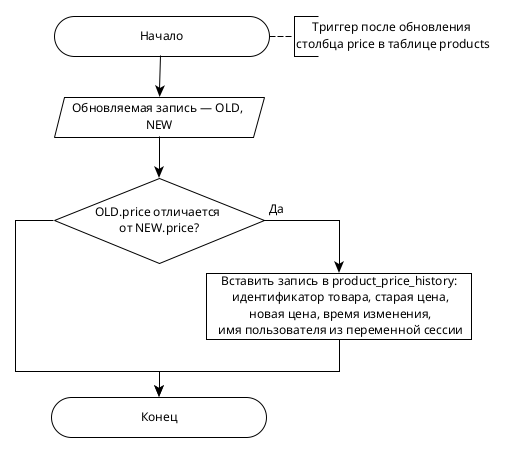
\includegraphics[width=0.7\textwidth]{img/trigger_catch_price_change.png}
    \caption{Схема алгоритма триггера аудита изменений цен}
    \label{fig:trigger_price}
\end{figure}

Триггер обеспечивает автоматическое формирование журнала изменения цен.

\subsection{Триггер пересчёта рейтингов}

Триггер \texttt{update\_ratings\_on\_review} активируется после вставки новой записи, обновления столбца \texttt{rating} или удаления записи в таблице \texttt{reviews}. Вызываемая функция \texttt{update\_product\_and\_seller\_rating} выполняет каскадный пересчёт:

\begin{enumerate}
    \item определяется идентификатор затронутого товара;
    \item рейтинг товара обновляется как среднее арифметическое оценок всех отзывов на данный товар (\texttt{AVG(rating)});
    \item по идентификатору продавца, полученному из обновлённой записи товара, пересчитывается рейтинг продавца как среднее арифметическое рейтингов всех его неудалённых товаров, имеющих хотя бы один отзыв.
\end{enumerate}

Схема алгоритма триггера приведена на рисунке~\ref{fig:trigger_rating}.

\begin{figure}[H]
    \centering
    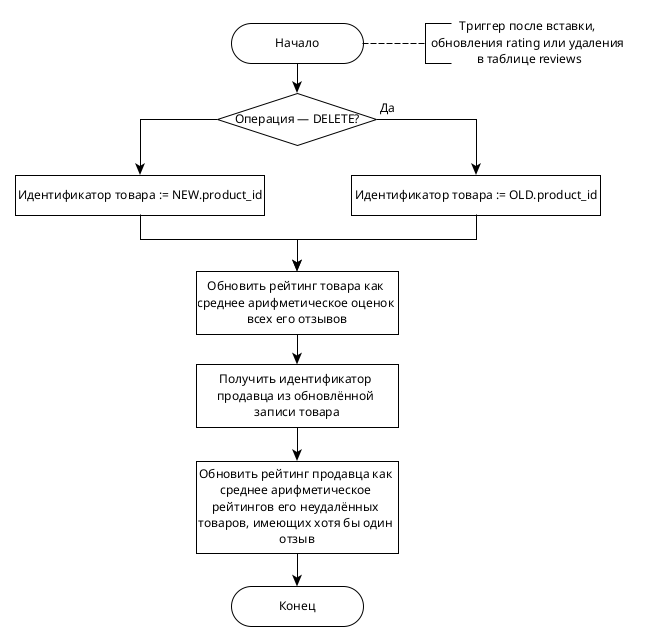
\includegraphics[width=0.7\textwidth]{img/trigger_update_ratings_on_review.png}
    \caption{Схема алгоритма триггера пересчёта рейтингов}
    \label{fig:trigger_rating}
\end{figure}

Такой подход поддерживает согласованность рейтингов: при добавлении, изменении или удалении отзыва автоматически обновляются рейтинги товара и продавца.

\subsection{Хранимая функция статистики продавца}

Функция \texttt{get\_seller\_statistics} принимает три параметра: идентификатор продавца (\texttt{p\_seller\_id}), начальную (\texttt{p\_date\_from}) и конечную (\texttt{p\_date\_to}) даты периода. Возвращает таблицу из четырёх столбцов:

\begin{itemize}
    \item \texttt{total\_orders} --- количество уникальных заказов;
    \item \texttt{total\_revenue} --- суммарная выручка;
    \item \texttt{avg\_order\_value} --- средний чек;
    \item \texttt{top\_product\_name} --- наименование самого продаваемого товара по количеству проданных единиц.
\end{itemize}

Функция объединяет данные таблиц \texttt{orders}, \texttt{order\_items} и \texttt{products} по идентификатору продавца и заданному временному интервалу. В расчёт включаются только заказы со статусами \texttt{paid}, \texttt{shipped} и \texttt{delivered}, что исключает из статистики неоплаченные и отменённые заказы.

Выручка рассчитывается как сумма произведений количества единиц товара на цену в момент покупки, что обеспечивает корректность подсчёта при наличии изменений цен. Средний чек вычисляется путём деления выручки на количество уникальных заказов.

Схема алгоритма функции приведена на рисунке~\ref{fig:function_stats}.

\begin{figure}[H]
    \centering
    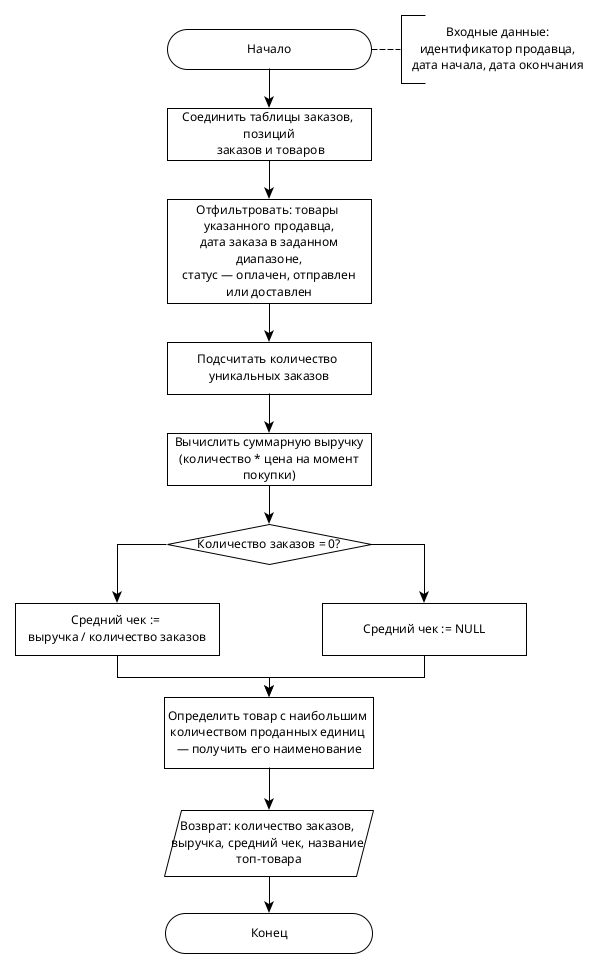
\includegraphics[width=0.7\textwidth]{img/function_get_seller_statistics.png}
    \caption{Схема алгоритма хранимой функции статистики продавца}
    \label{fig:function_stats}
\end{figure}


% !TEX root = ../../report.tex

\section{Проверка соответствия третьей нормальной форме}

Согласно требованиям к курсовой работе, спроектированная база данных должна находиться в третьей нормальной форме (3НФ). Отношение находится в 3НФ, если оно находится во второй нормальной форме и ни один неключевой атрибут не зависит транзитивно от первичного ключа~\cite{db_models}.

Проверка выполняется последовательно для каждой нормальной формы.

\subsection*{Первая нормальная форма (1НФ)}

Отношение находится в 1НФ, если все атрибуты содержат атомарные (неделимые) значения. В спроектированной базе данных это условие выполняется:

\begin{itemize}
    \item адрес доставки разделён на атомарные компоненты: \texttt{city}, \texttt{street}, \texttt{house}, \texttt{apartment}, \texttt{zip\_code};
    \item связь <<многие ко многим>> между товарами и категориями вынесена в отдельную таблицу \texttt{product\_categories};
    \item все остальные атрибуты содержат скалярные значения (строки, числа, даты, логические значения).
\end{itemize}

\subsection*{Вторая нормальная форма (2НФ)}

Отношение находится в 2НФ, если оно находится в 1НФ и каждый неключевой атрибут полностью функционально зависит от первичного ключа (отсутствуют частичные зависимости).

В большинстве таблиц первичным ключом является суррогатный идентификатор \texttt{id} (одноатрибутный ключ), при котором частичные зависимости невозможны по определению.

Единственная таблица с составным первичным ключом --- \texttt{product\_cate\-gories}. Ключ состоит из двух внешних ключей: \texttt{product\_id} и \texttt{category\_id}. Таблица не содержит неключевых атрибутов, следовательно, условие 2НФ выполняется тривиально.

\subsection*{Третья нормальная форма (3НФ)}

Отношение находится в 3НФ, если оно находится в 2НФ и не содержит транзитивных зависимостей неключевых атрибутов от первичного ключа.

Рассмотрим таблицы, в которых потенциально могут возникнуть транзитивные зависимости:

\begin{itemize}
    \item \textbf{orders}: атрибуты \texttt{user\_id}, \texttt{seller\_id} и \texttt{address\_id} являются внешними ключами, а не производными данными. Атрибут \texttt{total\_amount} может рассматриваться как вычисляемый (сумма позиций), однако хранится денормализованно для оптимизации выборок и фиксируется на момент оформления заказа;
    \item \textbf{products}: атрибут \texttt{rating} пересчитывается триггером на основе таблицы \texttt{reviews}. Формально это производное значение, хранимое для сокращения повторных расчётов рейтинга по отзывам. Атрибут \texttt{reserved\_quantity} хранит операционное состояние резерва товара и ограничивается условием \texttt{reserved\_quantity} $\leq$ \texttt{stock\_quantity};
    \item \textbf{sellers}: аналогично, \texttt{rating} пересчитывается триггером из рейтингов товаров.
\end{itemize}

Атрибуты \texttt{rating} в таблицах \texttt{products} и \texttt{sellers}, а также \texttt{total\_amount} в таблице \texttt{orders} представляют собой контролируемую денормализацию. Их значения должны поддерживаться в согласованном состоянии правилами проектируемой базы данных и правилами обработки заказов. Все остальные неключевые атрибуты зависят только от первичного ключа своей таблицы.

Таким образом, спроектированная база данных находится в третьей нормальной форме с обоснованной денормализацией вычисляемых агрегатов.

